\chapter{Review of papers}

\myminitoc

\sect{Sinkhorn Distances: Lightspeed Computation of Optimal Transport}

\cite{Cut}

\sect{Wasserstein GAN}

\cite{Arj++}

\sect{Convolutional Wasserstein Distances: Efficient Optimal Transportation on Geometric Domains \cite{Goe++}}

Because a single step of Sinkhorn algorithm has a complexity in $\mathcal{O}(n^2)$, computing the Wassertein distance may take a while in many cases. That's why the researchers who write this paper thought about a more effective solution to compute a step. They found a way to use Gaussian convolution with a $\mathcal{O}(n \log n)$ complexity instead of a matrix-vector product. More generally they use a heat kernel. So instead of the convolution it can also be a sparse pre-factored linear system which can be computed in a complexity smaller than $\mathcal{O}(n^2)$. Furthermore by doing this, the convergence is still linear. Of course this can not be applied in all cases of optimal transport, but it can be used on very common geometric domains, like images or meshes. In addition of the computation of Wasserstein distance, they also propose a way to use convolution in the computation of Wasserstein barycentres and Wasserstein propagation.

\paragraph{Using a heat kernel in the entropy-regularization}
We recall what is the entropy-regularized Wasserstein distance between $\mu_0$ and $\mu_1$ on the domain $M$:
$$ W_{2, \gamma}^2(\mu_0, \mu_1) = \inf_{\pi \in \Pi} \left[ \int \int_{M \times M} d(x, y)^2 \pi(x, y) dx dy \, - \, \gamma H(\pi) \right] = \gamma \left[ 1 + \min_{\pi \in \Pi} \text{KL}(\pi | \mathcal{K}_\gamma) \right]$$
Where:
$$ \Pi = \left\{ \pi \in \text{Prob}(M \times M) \, | \, \pi(\cdot, M) = \mu_0, \pi(M, \cdot) = \mu_1 \right\} $$
$$ H(\pi) = - \int \int_{M \times M} \pi(x, y) \ln \pi(x, y) dx dy $$
$$ \mathcal{K}_\gamma = e^{-d(x, y)^2 / \gamma} $$
$$ \text{KL}(\pi | \mathcal{K}) = \int \int_{M \times M} \pi(x, y) \left[ \ln \dfrac{\pi(x, y)}{\mathcal{K}(x, y)} - 1 \right]\ln  dx dy $$
This is a strictly convex problem thanks to the entropy. The idea of the paper is to use heat kernel because is some cases, the solution of the diffusion equation can be computed in a effective way. We denote by $\mathcal{H}_t(x, y)$ the diffusion between $x$ and $y$ after a time $t$ in the heat kernel. We have:
$$ \mathcal{K}_\gamma \approx \mathcal{H}_{\gamma / 2}(x, y) $$
We won't store $\mathcal{H}$ because it has a space complexity in $\mathcal{O}(n^2)$ and we want a lower complexity. But we generally know a way to apply $\mathcal{H}$ to a vector. In the case of images we apply Gaussian convolution with $\sigma^2 = \gamma$. \\
In the case of triangle meshes we associate a weight to faces proportional to their area. We denote by $a$ the vector of these weights (In images of size $n \times m$ we set $a = 1 / (nm)$). Then we denote by $L$ the cotangent Laplacian and by $D_a$ the diagonal matrix with diagonal $a$. By discretizing the heat equation, we obtain:
$$ w = \mathcal{H}_t(v) \Leftrightarrow \left( D_a + t L \right) w = v $$
The linear system can be solved efficiently by pre-computing a sparse Cholesky factorization.

\paragraph{Algorithm}
We some computations we arrive at:

\vspace{3mm}
\begin{algorithm}[H]
	\caption{\textsc{Convolutional-Sinkhorn}($\mu_0, \mu_1, H_t, a$)}
	$v, w \gets 1$ \;
	\Repeat{convergence of $v, w$}{
		$v \gets \mu_0 \oslash H_t(a \otimes w)$ \;
		$w \gets \mu_1 \oslash H_t(a \otimes v)$ \;
	}
	\Return $2t a^\trans \left[ \left( \mu_0 \otimes \ln v \right) + \left( \mu_1 \otimes \ln w \right) \right]$
\end{algorithm}
\vspace{3mm}

Where $\oslash$ and $\otimes$ denote element-wise operations. As Sinkhorn algorithm we obtain a simple iterative algorithm where, this time, steps can be computed in $\mathcal{O}(n \log n)$ in many cases, where $n$ is the size of the domain $M$.

\paragraph{Barycenter}
An algorithm for computing barycenters is also provided. We won't enter into details but we give their algorithm for computing the barycenter of distributions $\mu_i$ associated with weights $\alpha_i$ for $1 \leqslant i \leqslant k$:

\vspace{3mm}
\begin{algorithm}[H]
	\caption{\textsc{Convolutional-Barycenter}($\{\mu_i\}, \{ \alpha_i \}, H_t, a$)}
	$v_1, \dots, v_k \gets 1$ \;
	$w_1, \dots, w_k \gets 1$ \;
	\Repeat{convergence of $v_i, w_i$}{
		$\mu \gets 1$ \;
		\For{$i = 1, \dots, k$}{
			$w_i \gets \mu_i \oslash H_t(a \otimes v_i)$ \;
			$d_i \gets v_i \otimes H_t(a \otimes w_i)$ \;
			$\mu \gets \mu \otimes d_i^{\alpha_i}$ \;
		}
		\vspace{3mm}
		// Optional \;
		$\mu \gets $ \textsc{Entropic-Sharpening}$\left( \mu, \max_i H(\mu_i) \right)$ \;
		\vspace{3mm}
		\For{$i = 1, \dots, k$}{
			$v_i \gets v_i \otimes \mu \oslash d_i$ \;
		}
	}
	\Return $2t a^\trans \left[ \left( \mu_0 \otimes \ln v \right) + \left( \mu_1 \otimes \ln w \right) \right]$
\end{algorithm}
\vspace{3mm}
Where entropic sharpening allow us to make the entropy of the result $\mu$ smaller than the maximum entropy of all $\mu_i$. To do so if $H(\mu)$ is greater than $\max_i H(\mu_i)$, then we set $\mu$ to $\mu^\beta$ where $\beta$ is such that $H(\mu^\beta) = \max_i H(\mu_i)$. We can find $\beta$ using Newton's method.

\paragraph{Applications}
This has many applications in geometric domains. Applications that are given are:
\begin{itemize}
	\item Shape interpolation
		\begin{center}
		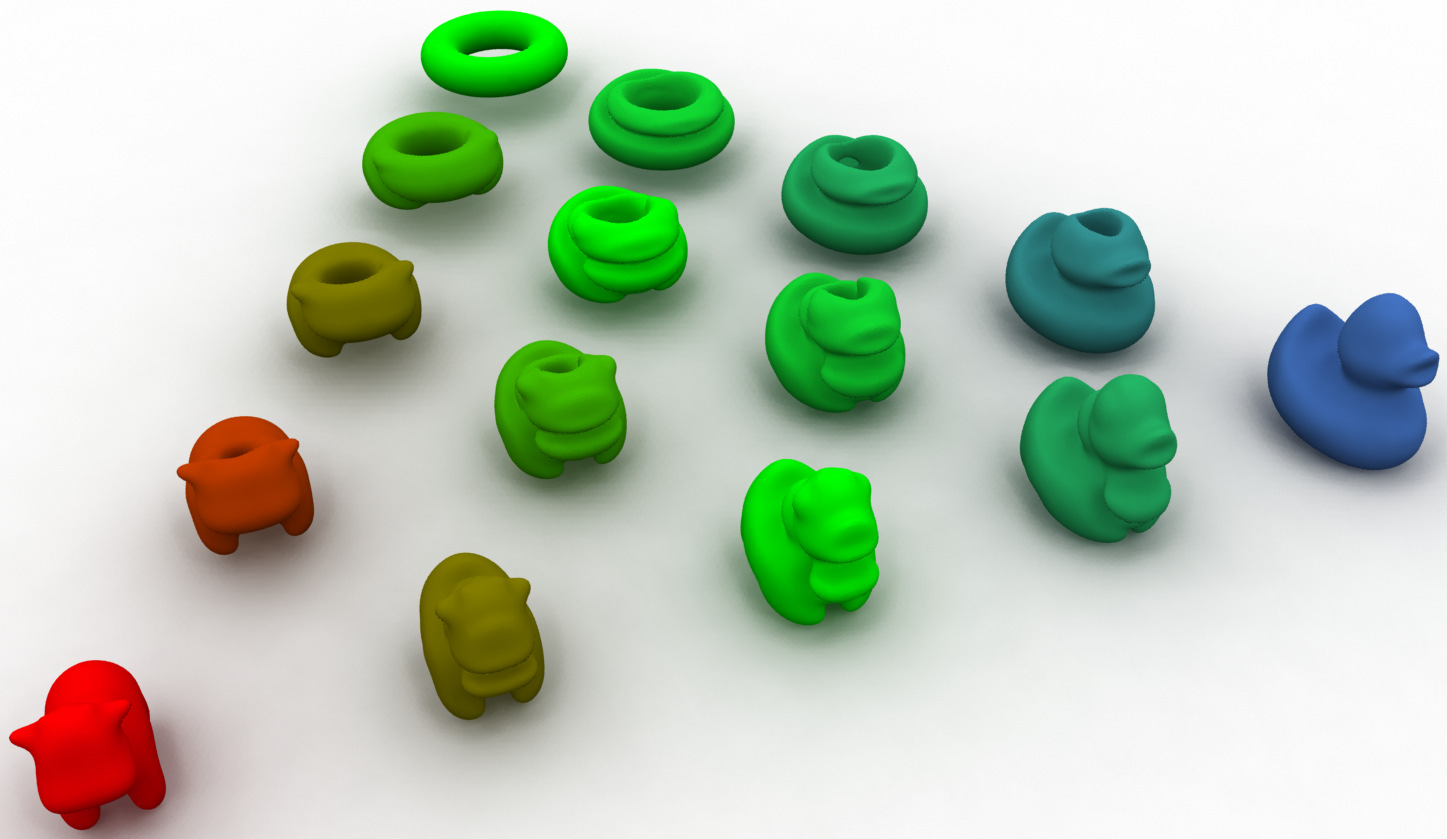
\includegraphics[scale=0.22]{shape_int.png}
		\end{center}
	\item BRDF design
	\item Color histogram manipulation
	\item Skeleton layout
	\item Soft maps
\end{itemize}
Finally here are two images of barycenters they have computed. The first one is an image where we find barycenters of four images that are in the corners. The second is an interpolation between two cards. As we tried to reproduce it in the implementation part we put them here :

\begin{center}
	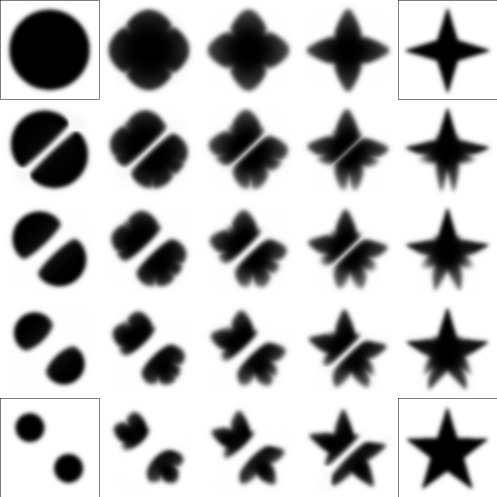
\includegraphics[scale=0.25]{bars_paper.png} \\ \vspace{3mm}
	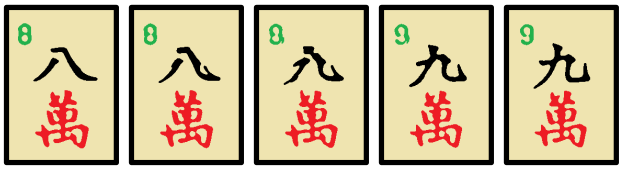
\includegraphics[scale=0.4]{cards_paper.png}
\end{center}